\section{Thrust 1. Predictive Code Coverage Analysis}
\label{sec:thrust1}

\subsection{{\cctool}: LLM Planning for Code Coverage Analysis}
\label{sec:approach_overview}



%\subsection{{\cctool} Workflow}
%\label{sec:approach_overview}
%{\cctool} exhibits a meticulously structured architecture tailored for the systematic prediction of test code coverage, employing a well-defined two-step approach, distinguished as The Plan Formation Module and The Coverage Prediction Module. Both the prompts (in a one-shot setting) have been illustrated in Figure 5(a) and Figure 5(b) respectively. The Plan Formation Module is tasked with predicting the step-by-step reasoning that the Large Language Model (LLM) must follow in order to predict the plan essential for subsequent coverage prediction of the provided test code. This plan, generated within the Plan Formation Module, serves as a pivotal component integrated into the Coverage Prediction Module and is employed to predict the code coverage of the given test code. Further elaboration of both modules is presented in the comprehensive sections below (refer to Figure 4) - 

%In Figure~\ref{fig:overview},

% Paragraph with overview-2
% This paper presents {\cctool} with two approaches to prompting: 
% a unified \textit{Plan}+\textit{Predict} design; and a two-phase
% \textit{Plan} $\xrightarrow{}$\textit{Predict} design.
% Figure~\ref{fig:overview} displays the workflow of \textit{Plan}
% $\xrightarrow{}$\textit{Predict}. For clarity, we do not show the
% unified version in which two prompts are consolidated including the
% examplary code, examplary plan, and given test code in
% Figure~\ref{fig:overview}.
%
% Paragraph with overview-3
This paper presents {\cctool} with two approaches to prompting: a
unified \textit{Plan}+\textit{Predict} design; and a two-phase
\textit{Plan} $\xrightarrow{}$\textit{Predict} design.
Figure~\ref{fig:codepilot} illustrates the workflow of both prompting
approaches.
%The general idea is that
For a given code snippet $C_T$ comprising the test input, {\cctool}
facilitates the systematic prediction of code coverage by formulating
a PA-based plan to navigate the code and attain an
understanding of its execution flow.  In the rest of the paper,
we refer to them as {\em one-prompt} and {\em two-prompt}
approaches,~respectively.
%Also, note that "Plan" corresponds to \textit{Plan Formulation} and "Predict" corresponds to \textit{Code Coverage Prediction}. 


\subsubsection{One-Prompt {\cctool}}
In this approach, for a given code snippet $C_T$ comprising the test inputs, {\cctool} facilitates the systematic prediction of code coverage by: [Step I. \textit{Plan Formulation}] constructing a plan rooted in program semantics to navigate the code and attain an understanding of the execution flow; [Step II. \textit{Code Coverage Prediction}] determining the code coverage based on such a plan. 

For this purpose, we leverage an LLM $\mathcal{M}_{CCP}^{I}$ that takes as an input prompt: (a) a set of instructions $\mathcal{I}_{CCP}$ describing the task; (b) an exemplar comprising code snippet $\mathcal{C}$ (different from $\mathcal{C}_T$), a manually-crafted, examplary plan $\mathcal{P}$, 
its code coverage $\mathit{Cov}$; and (c) the test code snippet $\mathcal{C}_T$.
Here, $\mathcal{M}_{CCP}^{I}$ utilizes the exemplar to guide the LLM to first reason about $C_T$ and construct a program semantics-guided code execution plan $P_T$, following which, it predicts the code coverage $\mathit{Cov}_T$.
This can be formulated as:
\begin{equation}
\langle \mathcal{P_T}, \textcolor{blue}{\mathit{Cov}_{T}} \rangle = \mathcal{M}_{CCP}^{I} \textbf{\ \{\ } \mathcal{I}_{CCP}, \langle \mathcal{C}, \mathcal{P}, \mathit{Cov} \rangle, \mathcal{C}_T \textbf{\ \}\ }  
\end{equation}



% We
% %present an overview of this workflow in Figure~\ref{fig:overview}, and
% will elaborate on two phases in Sections~\ref{sec:pfm}
% and~\ref{sec:cpm}, respectively. Section~\ref{sec:onephase} will
% explain the unified \textit{Plan}+\textit{Predict} design.
% %Alternatively, we also delegate the planning and code coverage
% %prediction tasks to the LLM in a single, consolidated prompt. Note
% %that, even both planning and actions are expressed in one prompt,
% %{\cctool} still consists of two phases because in the instruction, we
% %guide the LLM to produce the plan first and use it to predict code
% %coverage.

%We will elaborate on both prompting approaches in Sections~\ref{sec:plan+predict} and~\ref{sec:plan->predict}, respectively. We experiment with both One-Prompt and Two-Prompt solutions and compare their results (Section~\ref{rq1}).

%%\section{One-Prompt {\tool}}\label{sec:plan+predict}
%In this section, we present our design of the unified \textit{Plan}$+$\textit{Predict}.

\subsection{Basic Structure}
In the one-prompt setting (i.e., \textit{Plan}+\textit{Predict}), we design a single, consolidated prompt comprising three primary segments: (1) the instructions to the LLM to compute the code coverage for the given code snippet, (2) the exemplar(s) comprising code snippet, corresponding manually-crafted examplary plan, corresponding code coverage, and (3) the test code snippet. The output from the LLM includes: (1) the generated plan, and (2) the predicted code coverage for the test code snippet.

\subsubsection{Instructions}\label{sec:one-prompt-instructions} This segment contains specifications for the LLM to first generate a plan for understanding the execution flow in the given test code, using the manually-crafted plan for the code snippet in the exemplar(s) as a guide. Then, it instructs the LLM to follow the plan to compute the code coverage for the test code snippet, drawing parallels from the manually-crafted plan and the code coverage for the code snippet in the exemplar(s). Furthermore, the included code coverage guides the LLM to format the output code coverage prediction in the prescribed format.

\subsubsection{Exemplar(s)}\label{sec:one-prompt-structure} To guide the LLM as described in Section~\ref{sec:one-prompt-instructions}, we include example(s) for the few-shot setting comprising the code snippet, manually-crafted plan, and corresponding code coverage.

\subsubsection{Given Code Snippet} This is the code for which LLM~has to create a code execution plan and subsequently predict its coverage.

%The plan predicted by the LLM model when prompted in this step is
%then used later (Figure~\ref{sec:approach_overview}) to predict the
%coverage of the test code.



\subsection{Manually-Crafted Plan in Exemplar(s)}\label{sec:pfm_procedure-1}
The essence of designing the plan resides in the formulation of a step-by-step reasoning for understanding execution-flow in an exemplar code snippet. The structure of each step within the plan is composed of three fundamental elements: the step number, the type of statement(s), and the rationale behind their potential execution.

Firstly, the step numbers denote the sequence in which the code would have been executed. In Figure~\ref{fig:motiv-plan}(a), Step 4 (pertaining to the exemplar code in Figure~\ref{fig:motiv}(b)) labeled as `Main Method Execution' consistently follows Step 3, designated as `Main Method Call'.

Secondly, the label assigned to each step serves as the primary distinguishing factor for that set of statement(s) in the code. For example, the statements 18-19 in Figure~\ref{fig:motiv}(b) are categorized as `Variable Initialization' and are consequently grouped together in Step 7 of the exemplary plan in Figure~\ref{fig:motiv-plan}(a). It is noteworthy that certain labels, such as `Variable Initialization', `Method Call', `If-else Statement', among others, may directly indicate whether the associated statements will be executed. Details are given in Section~\ref{subsec:statement-types-1}.

%We will explain the details on different types of statements in Section~\ref{subsec:statement-types-1}.

Lastly, the final element of each step in the plan is the justification for the possible execution or non-execution of the
specific set of statements. For instance, let us consider Step 9 in Figure~\ref{fig:motiv-plan}(a), which analyzes the \code{if-else} statement in the \code{for} loop within the \code{main()} function (lines 20-22 of Figure~\ref{fig:motiv}(b)). Step 5 briefly explains that due to all the elements in list \code{A[]} being odd, only the condition in the \code{if} statement holds true, which leads to the statement(s) within the \code{if} branch to be executed. It also clearly mentions that since the condition of the \code{if} branch holds true through all iterations of the \code{for} loop, the \code{else} branch and its associated statements would have never been executed. This concise yet accurate reasoning is essential to guide the LLM to follow the step to design its own plan.

%\vspace{-4pt}
\subsection{Reasoning on Program Semantics}\label{subsec:statement-types-1}
To compute code coverage, the LLM needs to reason correctly on the execution steps of the statements in the code. In addition to the statements whose executions follow a sequential order, there are three types of statements that could {\em alter such  sequential execution}: {\em branching statements, loop statements, and method calls}.

In programming, the execution of branching statements (\code{if} or \code{switch} statements) are pivotal for controlling the flow of a program based on certain conditions. When encountering an \code{if} statement, the program evaluates a specified condition and, if true, executes the corresponding block of code; if false, it either moves to the next \code{elif} condition or proceeds to the \code{else} block if provided.
%This allows for branching and executing different code paths
%based on the evaluation of conditions. On the other hand,
In contrast, a \code{switch} statement is designed to evaluate an expression against multiple possible constant values. It provides a concise way to handle multiple cases, each with its own set of code. The exemplary plan needs to explain the nuances in the branching statements.  For example, the plan in Figure~\ref{fig:motiv-plan}(a) considers the \code{if-else} construct in the code snippet (Figure~\ref{fig:motiv}(b)) by briefly outlining the condition and the statement(s) executed based on the condition mentioned in the condition. This is expressed in Steps 6 and 9 of Figure~\ref{fig:motiv-plan}(a).

%The program compares the expression's value with each case and
%executes the block associated with the matching case. If no match is
%found, an optional `default` case can be executed. Both `if` and
%`switch` statements are powerful constructs that enhance the
%flexibility and logic of program execution.

%A code snippet can contain 3 blocks that are primarily responsible for a low accuracy in prediction - Branches, Loops and Methods. Branches contain all the possible 'if -else' blocks that a code snippet contains.  Loops consist of instructions iterated multiple times based on specified conditions. These include for, while, and do-while loops. Lastly, Methods are essentially functions that are bound to an object, and they can be called on that object to perform specific actions or operations.

The execution of a \code{for} statement and a \code{while} statement are both iterative processes.
%in programming.
The \code{for} statement is typically employed when the number of iterations is known beforehand. It consists of three~parts within its parentheses: initialization, condition, and increment/decrement. The loop executes as long as the specified condition remains true. In contrast, a \code{while} statement is more versatile and is used when the number of iterations is uncertain or depends on a certain condition. The \code{while} loop continues to execute as long as the specified condition holds true, and the programmer is responsible for updating the loop variable within the loop block. While both constructs facilitate iteration, the \code{for} statement is more structured and concise, while the \code{while} statement offers greater flexibility in handling variable loop conditions. Such nuances of a loop statement need to be incorporated into the exemplar plan. For example, let us consider Step 5 of Figure~\ref{fig:motiv-plan}(a). The plan for the exemplary code snippet in Figure~\ref{fig:motiv}(b) explains the number of iterations for each of the statements in the \code{for} loop. Since the \code{for} loop is not conditional, line 21 in Figure~\ref{fig:motiv}(b) will be executed.
%
Lastly, the plan also includes the reason behind the execution of a statement containing a method call. Upon calling a method, the plan progresses to the subsequent step, involving the execution of the called method.

In addition to the statement-specific guiding, the exemplary plan accommodates additional statements found in a code snippet, such as variable initialization and print statements. This can be seen in Steps 1, 4 and 12 of Figure~\ref{fig:motiv-plan}(a), which have been created primarily for accommodating the package import statements, variable initialization within a method and print statements, respectively.

%In addition to handling the three primary blocks, the plan accommodates supplementary statements found in a code snippet, such as variable initialization and print statements. This can be seen in Steps 1, 4 and 12 of Figure 2(a), which have been created with the primary aim of accommodating the package import statements, variable initialization within a method and print statements respectively. 

\subsection{Illustrating Example}\label{sec:one-prompt-ex}

%\begin{figure}[t]
\begin{wrapfigure}{r}{0.65\textwidth}
	\centering
	\lstset{
		numbers=left,
		numberstyle= \tiny,
		keywordstyle= \color{blue!70},
		commentstyle= \color{red!50!green!50!blue!50},
		frame=shadowbox,
		rulesepcolor= \color{red!20!green!20!blue!20} ,
		xleftmargin=1.5em,xrightmargin=1em, aboveskip=1em,
		framexleftmargin=1.5em,
                numbersep= 5pt,
		language=Python,
    basicstyle=\tiny\ttfamily,
    numberstyle=\tiny\ttfamily,
    emphstyle=\bfseries,
                moredelim=**[is][\color{red}]{@}{@},
		escapeinside= {(*@}{@*)}
	}
\begin{minipage}{.45\textwidth}        
\begin{lstlisting}[caption = ]
(*@{\color{red}{ONE-PROMPT SETTING@*)
For the given code snippet, Predict the code coverage. The code coverage indicates whether a statement has been executed (*@\color{black}{or not}@*). 
> (*@\color{black}{if}@*) the line (*@\color{black}{is}@*) executed
! (*@\color{black}{if}@*) the line (*@\color{black}{is not}@*) executed

Example output:
> line1
! line2
> line3
...
> linen

You need to develop a plan (*@\color{black}{for}@*) step by step execution of the code snippet. 
Below (*@\color{black}{is}@*) an illustration of the process you need to follow to predict the code coverage of the given code snippet. 

(*@\color{orange}{Example - Given Code Snippet:}@*) 
number = 15
if number % 2 == 0:
    print("{} is an even number.".format(number))
else:
    print("{} is an odd number.".format(number))

(*@\color{orange}{PLAN :}@*) 
Step 1: Variable Initialization: Initialize the number variable with a specific value. In this case, it(*@\color{black}{'}@*)s (*@\color{black}{set}@*) to 15. Statements "number = 15" will be executed. "if number % 2 == 0:" will be executed
Step 2: Operation : Use the % (modulo) operator to check (*@\color{black}{if}@*) the number (*@\color{black}{is}@*) divisible by 2. If the result (*@\color{black}{is}@*) 0, the number (*@\color{black}{is}@*) even. If (*@\color{black}{not}@*), it(*@\color{black}{'}@*)s odd.
Step 3: Branching (*@\color{black}{if-else}@*) Block: Enter the if block (*@\color{black}{if}@*) the number (*@\color{black}{is}@*) even. Since 15%2 results (*@\color{black}{in}@*) 1, statement "print("{} (*@\color{black}{is}@*) an even number.".format(number))" will (*@\color{black}{not}@*) be executed but the else block will (*@\color{black}{if}@*) the number (*@\color{black}{is}@*) odd. Statements "else:" (*@\color{black}{and}@*) "print("{} (*@\color{black}{is}@*) an odd number.".format(number))" will be executed
Step 4: Output: The required print statement will be executed based on the output of the if-else block

(*@\color{orange}{So the code coverage for the given code snippet will be:}@*) 
> from math import factorial
> number = 15
> if number % 2 == 0:
!     print("{} is an even number.".format(number))
> else:
>     print("{} is an odd number.".format(number))

In a similar fashion, develop a plan of step by step execution of the below code snippet (*@\color{black}{and}@*) predict the code coverage - 
(*@{\color{red}{<< Test Code... >>@*)
\end{lstlisting}
\end{minipage}
\vspace{-18pt}
\caption{Example on one-prompt setting with {\tool}}
\label{fig:one-prompt}
\end{wrapfigure}


The example presented in Figure~\ref{fig:one-prompt} outlines the process of predicting code coverage using one-prompt {\tool} for a given code snippet. The objective is to first predict a plan for the test code, and then determine the executed or non-executed status of each line, denoted by '>' for executed lines and '!' for non-executed lines. The detailed instruction is illustrated in lines 2--11.

The example code snippet (lines 18-22 of Figure~\ref{fig:one-prompt}) initializes a variable \code{number} to \code{15}, followed by a conditional statement checking if the number is even or odd. The provided plan (lines 25-28) details the execution steps, such as variable initialization, modulo operation, branching in the \code{if-else} block, and the corresponding output. Following the outlined steps, the final predicted code coverage is presented (lines 31--36), highlighting the lines that are expected to be executed or skipped based on the given plan.
%This approach facilitates a systematic assessment of code
%coverage, aiding in the evaluation and understanding of the test
%code's execution flow.
The subsequent request prompts a similar analysis for a different test code (line 40 onwards), encouraging a comprehensive exploration of code coverage prediction within the generated plan.




%\section{Two-Prompt \tool}\label{sec:plan->predict}
In this section, we present our design of the two-phase \textit{Plan} $\xrightarrow[]{}$\textit{Predict}.

\subsection{Plan Formulation}
\subsubsection{Basic Structure}
This section presents the first phase, i.e., \textit{Plan Formulation}, in \textit{Plan} $\xrightarrow{}$\textit{Predict}. In this phase, we design a prompt comprising three primary segments: (1) instructions to the LLM to devise a PA-based plan, (2) exemplar(s) comprising code snippet and corresponding plans, (3) test code snippet. The output from the LLM comprises of the generated plan for the test code snippet.

%The Plan Formation Module is the first segment of {\tool} and is responsible for the prediction of the step by step reasoning process that will later be essential to predict the code coverage of the given test code. Functioning as a singular prompt, the module comprises multiple segments, each holding equal significance and contributing indispensably to the Plan's prediction. The comprehensive breakdown of this module as follows :

%\subsection{\bf Basic Architecture}
%\label{sec:pfm_architecture}

\subsubsection*{Instructions} The first segment consists of the problem statement explained in natural language, which instructs the LLM to predict/build its own plan to be pursued for predicting the code coverage of the given
test code (see example in Section~\ref{sec:pfm_example-2}).

\subsubsection*{Exemplar(s)}
\label{subsec:examplar}
%Also known as The Reasoning Prompt, this segment of {\tool} comprises 3 sections, as depicted in Figure 4. The first section consists of the problem statement presented in natural language, which instructs the LLM to predict the plan to be pursued for the prediction of code coverage in the given test code. {\color{red}DOUBT : include a figure showing the prompt for the plan prediction!!!}
The second segment of the prompt incorporates exemplar(s) to enable the few-shot setting, each comprising a code snippet (distinct from the given test code) and a manually-crafted plan. Each step within that plan provides a succinct elucidation of the reasons behind the (non)-execution of the associated statement(s). The procedure for crafting the plan is same as in Section~\ref{sec:pfm_procedure-1}. The LLM uses this as a guide to understand the execution flow.

%Using this as a guide, the LLM predicts a plan for understanding the execution-flow in the test code snippet.

\subsubsection*{Given Test Code Snippet}
\label{subsec:testcode}
The last segment is the test code for which LLM has to create the code execution plan. 

\subsubsection{Illustrating Example}\label{sec:pfm_example-2}
\begin{figure}[t]
	\centering
	\lstset{
		numbers=left,
		numberstyle= \tiny,
		keywordstyle= \color{blue!70},
		commentstyle= \color{red!50!green!50!blue!50},
		frame=shadowbox,
		rulesepcolor= \color{red!20!green!20!blue!20} ,
		xleftmargin=1.5em,xrightmargin=1em, aboveskip=1em,
		framexleftmargin=1.5em,
                numbersep= 5pt,
		language=Python,
    basicstyle=\tiny\ttfamily,
    numberstyle=\tiny\ttfamily,
    emphstyle=\bfseries,
                moredelim=**[is][\color{red}]{@}{@},
		escapeinside= {(*@}{@*)}
	}
\hspace{8pt}
% \begin{minipage}{.45\textwidth}        
% \begin{lstlisting}[caption = ]
% (*@{\color{red}{PLAN FORMATION MODULE}@*)
% For the given code snippet, give the plan to predict the code coverage. The code coverage indicates whether a statement has been executed (*@\color{black}{or not.}@*) 

% You need to develop a plan (*@\color{black}{for}@*) step by step execution of the code snippet. 
% Below (*@\color{black}{is}@*) an illustration of the process you need to follow to predict the code coverage of the given code snippet. 

% (*@\color{orange}{Example -}@*) 
% (*@\color{orange}{Given Code snippet :}@*)
% number = 15
% if number % 2 == 0:
%     print("{} is an even number.".format(number))
% else:
%     print("{} is an odd number.".format(number))

% (*@\color{orange}{PLAN :}@*)
% Step 1: Variable Initialization: Initialize the number variable with a specific value. In this case, it(*@\color{black}{'}@*)s (*@\color{black}{set}@*) to 15. Statements "number = 15" will be executed. "if number % 2 == 0:" will be executed
% Step 2: Operation : Use the % (modulo) operator to check (*@\color{black}{if}@*) the number (*@\color{black}{is}@*) divisible by 2. If the result (*@\color{black}{is}@*) 0, the number (*@\color{black}{is}@*) even. If (*@\color{black}{not}@*), it(*@\color{black}{'}@*)s odd.
% Step 3: Branching (*@\color{black}{if-else}@*) Block: Enter the if block (*@\color{black}{if}@*) the number (*@\color{black}{is}@*) even. Since 15%2 results (*@\color{black}{in}@*) 1, statement "print("{} (*@\color{black}{is}@*) an even number.".format(number))" will (*@\color{black}{not}@*) be executed but the else block will (*@\color{black}{if}@*) the number (*@\color{black}{is}@*) odd. Statements "else:" (*@\color{black}{and}@*) "print("{} (*@\color{black}{is}@*) an odd number.".format(number))" will be executed
% Step 4: Output: The required print statement will be executed based on the output of the if-else block

% In a similar fashion, develop a plan of step by step execution of the below code snippet - 
% (*@{\color{red}{<< Test Code... >>}@*)

% \end{lstlisting}
% \vspace{-9pt}
% \subcaption{One-shot Prompt used in Plan Formation}
% \label{fig:example-plan-formation}
% \end{minipage}
\begin{minipage}{.45\textwidth}        
\begin{lstlisting}[caption = ]
(*@{\color{red}{PLAN FORMATION}@*)
For the given code snippet, give the plan to predict the code coverage. The code coverage indicates whether a statement has been executed (*@\color{black}{or not.}@*) 

You need to develop a plan (*@\color{black}{for}@*) step by step execution of the code snippet. 
Below (*@\color{black}{is}@*) an illustration of the process you need to follow to predict the code coverage of the given code snippet. 

(*@\color{red}{<< Exemplar code, as on Lines 16-22 in Figure 5 >>}@*) 

(*@\color{red}{<< Exemplar plan, as on Lines 24-28 in Figure 5 >>}@*) 

In a similar fashion, develop a plan of step by step execution of the below code snippet - 
(*@{\color{red}{<< Test Code... >>}@*)

\end{lstlisting}
\vspace{-9pt}
\subcaption{One-shot prompt used for \textit{Plan Formation}}
\label{fig:example-plan-formation}
\end{minipage}
%\hspace{8pt}
% \begin{minipage}{.45\textwidth}        
% \begin{lstlisting}[caption = ]
% (*@{\color{red}{COVERAGE PREDICTION MODULE}@*)
% For the given code snippet (*@\color{black}{and}@*) plan, give the code coverage that follows the plan. The code coverage indicates whether a statement has been executed (*@\color{black}{or not}@*). 
% > (*@\color{black}{if}@*) the line (*@\color{black}{is}@*) executed
% ! (*@\color{black}{if}@*) the line (*@\color{black}{is not}@*) executed
% Example output:
% > line1
% ! line2
% > line3
% ...
% > lineN
% You need to give the code with its coverage (*@\color{black}{for}@*) the given plan.
% Below (*@\color{black}{is}@*) an illustration of the process you need to follow to predict the code coverage of the given code snippet (*@\color{black}{and}@*) its plan. 
% (*@\color{orange}{Given Code snippet :}@*) 
% number = 15
% if number % 2 == 0:
%     print("{} is an even number.".format(number))
% else:
%     print("{} is an odd number.".format(number))
% DISCLAIMER: Lines that are not executed are to be denoted with a SINGLE '!' whereas lines that are executed are to be denoted with a single '>'

% (*@\color{orange}{Given PLAN :}@*) 
% Step 1: Variable Initialization: Initialize the number variable with a specific value. In this case, it(*@\color{black}{'}@*)s (*@\color{black}{set}@*) to 15. Statements "number = 15" will be executed. "if number % 2 == 0:" will be executed
% Step 2: Operation : Use the % (modulo) operator to check (*@\color{black}{if}@*) the number (*@\color{black}{is}@*) divisible by 2. If the result (*@\color{black}{is}@*) 0, the number (*@\color{black}{is}@*) even. If (*@\color{black}{not}@*), it(*@\color{black}{'}@*)s odd.
% Step 3: Branching (*@\color{black}{if-else}@*) Block: Enter the if block (*@\color{black}{if}@*) the number (*@\color{black}{is}@*) even. Since 15%2 results (*@\color{black}{in}@*) 1, statement "print("{} (*@\color{black}{is}@*) an even number.".format(number))" will (*@\color{black}{not}@*) be executed but the else block will (*@\color{black}{if}@*) the number (*@\color{black}{is}@*) odd. Statements "else:" (*@\color{black}{and}@*) "print("{} (*@\color{black}{is}@*) an odd number.".format(number))" will be executed
% Step 4: Output: The required print statement will be executed based on the output of the if-else block

% (*@\color{orange}{So the final code coverage will be :}@*) 
% > number = 15
% > if number % 2 == 0:
% !     print("{} is an even number.".format(number))
% > else:
% >     print("{} is an odd number.".format(number))

% In a similar fashion, Give the code coverage of the below code snippet based on the given plan - 

% (*@{\color{red}{<< Test Code... >>}@*)
% (*@{\color{red}{Plan generated in Plan Formation Phase}@*)

% \end{lstlisting}
% \vspace{-9pt}
% \subcaption{One-shot Prompt used in Coverage Prediction}
% \label{fig:example-plan-cc-prediction}
% \end{minipage}
\begin{minipage}{.45\textwidth}        
\begin{lstlisting}[caption = ]
(*@{\color{red}{COVERAGE PREDICTION}@*)
For the given code snippet (*@\color{black}{and}@*) plan, give the code coverage that follows the plan. The code coverage indicates whether a statement has been executed (*@\color{black}{or not}@*). 
> (*@\color{black}{if}@*) the line (*@\color{black}{is}@*) executed
! (*@\color{black}{if}@*) the line (*@\color{black}{is not}@*) executed
Example output:
> line1
! line2
> line3
...
> lineN
You need to give the code with its coverage (*@\color{black}{for}@*) the given plan.
Below (*@\color{black}{is}@*) an illustration of the process you need to follow to predict the code coverage of the given code snippet (*@\color{black}{and}@*) its plan. 
(*@\color{red}{<< Exemplar code, as on Lines 16-22 in Figure 5 >>}@*) 

DISCLAIMER: Lines that are not executed are to be denoted with a SINGLE '!' whereas lines that are executed are to be denoted with a single '>'

(*@\color{red}{<< Exemplar plan, as on Lines 24-28 in Figure 5 >>}@*) 

(*@\color{red}{<< Exemplar code coverage, as on Lines 30-36 in Figure 5 >>}@*) 

In a similar fashion, give the code coverage of the below code snippet based on the given plan - 

(*@{\color{red}{<< Test code... >>}@*)
(*@{\color{dkgreen}{<< Test plan (generated by the Plan Formulation phase)... >>}@*)

\end{lstlisting}
\vspace{-9pt}
\subcaption{One-shot prompt used for \textit{Code Coverage Prediction}}
\label{fig:example-plan-cc-prediction}
\end{minipage}
\vspace{-9pt}
\caption{Prompts with a single exemplar (i.e., one-shot) for \textit{Plan Formulation} (top) and \textit{Code Coverage Prediction} (bottom) phases in two-prompt {\tool}.}
\label{fig:example}
\end{figure}

An example prompt for the \textit{Plan Formulation} phase is provided with a single exemplar in Figure~\ref{fig:example}(a). 
Note that the code snippet and the corresponding manually-crafted plan in the exemplar are the same as in Section~\ref{sec:one-prompt-ex}. 

Similar to as in one-prompt {\tool}, the prompt in this phase guides the LLM to draw parallels from the execution rationale in the exemplar plan by learning to reason about the exemplar code, and subsequently, generate a similar plan for the test code. Such a break down of the test code into comprehensible steps enables the LLM to reason about the code execution and make predictions regarding which statements will be executed or skipped. Thus, such a systematic approach encapsulated within the \textit{Plan Formulation} phase instills a structured method for later predicting the code coverage. By design, this approach provides a guide to understand the code coverage prediction, improving the LLM's interpretability.
%
% Already included in Section 4.4 now.
%
% First, the module directs the initialization of the
% \code{number} variable to a specific value (15), ensuring the
% execution of the corresponding statement. Subsequently, the modulo
% operator is employed to assess the divisibility of \code{number} by
% 2. Based on the result, the plan dictates the branching of the
% execution into either the \code{if} block or the \code{else} block. As
% the execution progresses through the plan, we guide the model to
% predict whether specific statements within the code snippet will be
% executed or not. For example, in the given scenario, the plan predicts
% that the print statement within the \code{if} block will not be
% executed due to the specific value of \code{number}. However,
% statements within the \code{else} block will be executed.
%
% This systematic approach, encapsulated in the plan formation phase,
% instills a structured method for later predicting code coverage. The
% module's process involves breaking down the code snippet into
% comprehensible steps, enabling the LLM to reason about the execution
% steps and make predictions regarding which statements will be executed
% or skipped. This approach is not only expected to enhance the LLM's
% interpretability but also provides a valuable guide for predicting the
% code coverage in the later phase.



\subsection{Code Coverage Prediction}

\subsubsection{Basic Structure}
This section presents the second phase, i.e., \textit{Code Coverage Prediction}, in \textit{Plan} $\xrightarrow{}$\textit{Predict}. In this phase, we design a prompt comprising four primary segments: (1) instructions to the LLM to compute the code coverage for the code snippet, (2) exemplar(s) comprising code snippet, corresponding manually-crafted exemplary plan and code coverage, (3) test code snippet, (4) generated plan from \textit{Plan Formulation} phase. The output from the LLM comprises the predicted code coverage for the given test code.

\subsubsection*{Instructions} This segment in the second prompt requests the LLM to adhere to the {\em generated plan} to predict the code coverage for the given test code, using the exemplar(s) to guide this process. 

\subsubsection*{Exemplar(s)} In the two-prompt setting, the exemplar(s) are exactly the same as in one-prompt {\tool} (see Section~\ref{sec:one-prompt-structure}). The inclusion of this serves the purpose of guiding the LLM towards achieving a code coverage prediction in the prescribed format.

\subsubsection*{Given Test Code Snippet} This segment is same in both \textit{Plan Formulation} (Section~\ref{subsec:testcode}) and \textit{Code Coverage Prediction} phases.

\subsubsection*{Generated Plan} In the two-prompt setting, the plan generated from the \textit{Plan Formulation} phase is incorporated into the prompt in this phase to guide the code coverage prediction. Note that this differs from the one-prompt {\tool} where one LLM is tasked with generating both the plan and the code coverage sequentially.

\subsubsection{Illustrating Example}\label{cpm_example-2}
An example prompt for the \textit{Code Coverage Prediction} phase is provided with a single exemplar in Figure~\ref{fig:example-plan-cc-prediction}. Note that the exemplar's structure is same as that in one-prompt {\tool}, including the same code snippet and manually-crafted plan in the exemplar as in the \textit{Plan Formulation} phase (Section~\ref{sec:plan->predict}), as well as the corresponding code coverage. Next, along with the test code, we include the test plan generated in the \textit{Plan Formulation} phase. By design, this prompt facilitates the 
prediction of code coverage for the test code from the generated plan, inherently learning such associations between alike components in the exemplar(s).

% The example presented in Figure~\ref{fig:example-plan-cc-prediction} outlines the process of predicting code coverage using the code coverage prediction within the context of a given code snippet and its plan. The objective is to determine the executed or non-executed status of each line, denoted by '>' for executed lines and '!' for non-executed lines. The detailed instruction is illustrated in lines 2--12.

% The example code snippet (lines 14-18 of
% Figure~\ref{fig:example-plan-cc-prediction}(b)) initializes a
% variable, 'number,' to 15, followed by a conditional statement
% checking if the number is even or odd. The provided plan (lines 21-25)
% details the execution steps, such as variable initialization, modulo
% operation, branching in the \code{if-else} block, and the
% corresponding output. Following the outlined steps, the final
% predicted code coverage is presented (lines 26--31), highlighting the
% lines that are expected to be executed or skipped based on the given
% plan.
% %This approach facilitates a systematic assessment of code
% %coverage, aiding in the evaluation and understanding of the test
% %code's execution flow.
% The subsequent request prompts a similar analysis for a different test
% code (lines 33 - 35), encouraging a comprehensive exploration of code
% coverage prediction within the generated plan.



\subsubsection{Two-Prompt {\cctool}}
%For a given code snippet $C_T$ comprising the test inputs, {\cctool} facilitates the systematic prediction of code coverage by employing two phases: \textit{Plan Formulation}, and \textit{Code Coverage Prediction}.

\begin{figure}[t] 
    \centering
%    \includegraphics[width=3.4in]{diagrams/overview-2.png}
    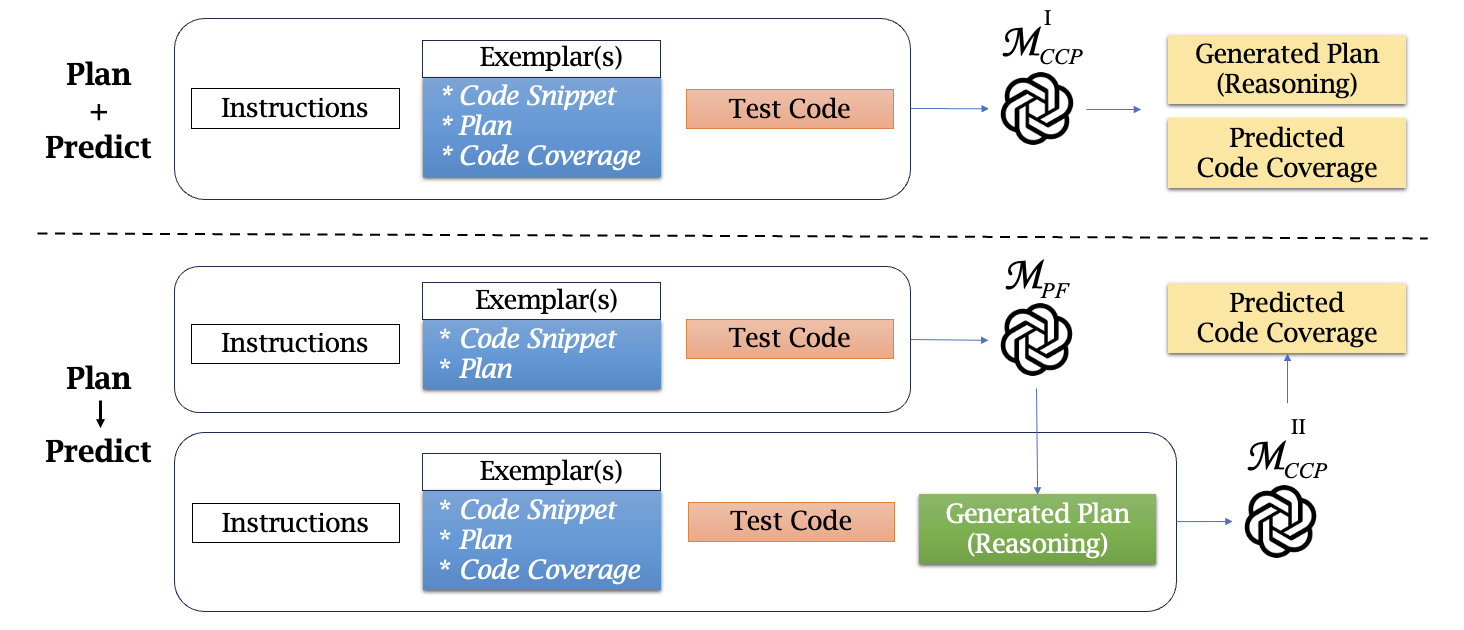
\includegraphics[width=0.7\linewidth]{codepilot-overview.png}
    \vspace{-19pt}
    \caption{Overview of {\cctool} Workflow for \textit{One-Prompt} (top) and \textit{Two-Prompt} (bottom) settings.}
    \label{fig:codepilot}
\end{figure}

Unlike in one-prompt {\cctool}, in this approach, we divide both \textit{Plan Formulation} and \textit{Code Coverage Prediction} in two prompts. The goal of the initial \textit{Plan Formulation} phase is to guide the LLM to \underline{\textit{reason}} about the given code snippet and construct a plan by itself, that is integral for navigating the code snippet and attaining an understanding of the execution flow. For this purpose, we leverage an LLM $\mathcal{M}_{PF}$ that takes as an input prompt: (a) a set of instructions $\mathcal{I}_{PF}$ describing the task; (b) an exemplar comprising a code snippet $\mathcal{C}$ (different from $\mathcal{C}_T$) and its corresponding plan $\mathcal{P}$; (c) the given code snippet $\mathcal{C}_T$. 
Here, $\mathcal{M}_{PF}$ utilizes the exemplar to guide the LLM to generate a similar plan $\mathcal{P}_T$ for $\mathcal{C}_T$.
%Let the LLM-generated plan for $\mathcal{C}_T$ be $\mathcal{P}_T$. 
This can be formulated as:
\begin{equation}\label{form:f1}
\textcolor{dkgreen}{\mathcal{P}_T} = \mathcal{M}_{PF} \textbf{\ \{\ } \mathcal{I}_{PF}, \langle \mathcal{C}, \mathcal{P} \rangle, \mathcal{C}_T \textbf{\ \}\ }  
\end{equation}

In \textit{Code Coverage Prediction} phase, the goal is to \underline{\textit{act}} on the code snippet $\mathcal{C}_T$ as per the LLM-generated plan $\mathcal{P}_T$ to enhance its execution-flow understanding, and predict the code coverage accordingly. For this purpose, we leverage an LLM $\mathcal{M}_{CCP}^{II}$ that takes as an input prompt: (a) a set of instructions $\mathcal{I}_{CCP}$ describing the task; (b) an exemplar comprising code snippet $\mathcal{C}$ and its plan $\mathcal{P}$ (same as in the \textit{Plan Formulation} phase), as well as its code coverage $\mathit{Cov}$; (c) the test code snippet $\mathcal{C}_T$; and (d) the LLM-generated plan $\mathcal{P}_T$.
Here, $\mathcal{M}_{CCP}^{II}$ utilizes the exemplar to guide the LLM to learn to determine the code coverage for the code example based on the program semantics-guided code execution plan. Subsequently, based on the $\mathcal{M}_{PF}$-generated plan $\mathcal{P}_T$ for the test code snippet, it predicts the code coverage $\mathit{Cov}_T$. 
This can be formulated as:
\begin{equation}
\textcolor{blue}{\mathit{Cov}_{T}} = \mathcal{M}_{CCP}^{II} \textbf{\ \{\ } \mathcal{I}_{CCP}, \langle \mathcal{C}, \mathcal{P}, \mathit{Cov} \rangle, \mathcal{C}_T, \textcolor{dkgreen}{\mathcal{P}_T} \textbf{\ \}\ }  
\end{equation}

\subsection{CFG-based Planning for Code Coverage Prediction}

%\subsection{Key ideas}

We aim to introduce a novel planning framework for code
execution, named \underline{O}bservation, \underline{R}easoning, and
\underline{C}ode-Driven, \underline{A}ction ({\orca}). {\orca} prompts
the GPT~\cite{chatGPT} to autonomously devising a plan for
predictive execution by traversing the CFG and
subsequently detecting the runtime errors.

\subsubsection{Teaching the LLM to `execute' the CFG}

%Guiding a model to navigate and predict the execution within a CFG
%offers advantages in mitigating the limitations of the aforementioned
%rudimentary approach, which dissects loop execution into
%fragments. Initially, despite segmenting execution into blocks,
%continuity of variable values from one block to the next can be
%preserved. This is reinforced by employing a "symbol table" to monitor
%relevant variable values within the current loop context. Secondly,
%traversing a cycle within the CFG mirrors iteration through the
%corresponding loop in the source code, while branching conditions in
%the CFG signify loop entry and exit criteria. Thirdly, edges
%connecting the blocks inherently depict control flows dictated by
%flow-altering statements. For instance, the \code{continue} statement
%at line 6 of Fig.~\ref{fig:motiv} is depicted by the edge labeled with '*' in Fig.~\ref{fig:cfg}.

Guiding a model to traverse and predict the execution in a CFG
provides benefits to address the issues with the above naive solution,
which `executes' a loop by breaking it up into fragments. First,
despite breaking the `execution' into CFG blocks, the propagation of the
values in the context of the previous block can be maintained. To
reinforce this, we leverage the usage of a {\em symbol table} that
tracks the variable values relevant to the current block. Second, the
traversal through a circle in the CFG corresponds to the iterating
through the corresponding loop in the source code, and the branching
condition in the CFG represents the loop-entering and loop-exiting
conditions. Third, the edges among the blocks automatically represent
the control flows that are decided by the flow-altering
statements, e.g., \code{continue}, etc.

%For example, the \code{continue} statement at line 6 of
%Fig.~\ref{fig:motiv} is represented by the edge marked by `*' in
%Fig.~\ref{fig:cfg}.


\subsubsection{Leveraging LLM-based Planning on CFG}

%Automated planning capability of a LLM is the ability to develop an
%efficient and effective process to generate plans or sequences of
%actions to break down a complex task to achieve a goal into smaller
%and manageable
%steps~\cite{valmeekam2023on,pallagani2023understanding}. Researchers
%have proposed different planning frameworks for LLMs to effectively
%tackle a range of tasks in several domains~\cite{tien}.

The automated planning capacity of an LLM refers to its adeptness in
devising a streamlined and productive method for crafting plans or
sequences of actions. These plans are designed to deconstruct a
complex task, enabling the achievement of a goal through a series of
smaller, manageable
steps~\cite{valmeekam2023on,pallagani2023understanding}. Researchers
have introduced diverse planning frameworks tailored for LLMs,
facilitating their effective handling of a multitude of tasks in
various
domains~\cite{zhuang2024toolchain,hu2023avis,yao2023react,prasad2023adapt}.
%
%In the planning techniques, reasoning traces assist the LLMs in
%deducing, monitoring, and refining action plans, while actions
%facilitate interaction with external sources, such as
%environments~\cite{prasad2023adapt,yao2023react}.
The planning techniques have demonstrated efficacy in mitigating
issues like hallucination and error propagation in LLMs when tackling
complex tasks~\cite{yao2023react}.

%We aim to leverage LLM planning to guide it to devise a plan that
%`executes' the code by walking through the CFG and dynamically decides
%the paths through the conditions. Specifically, we adapted
%ReAct~\cite{yao2023react} to our problem. ReAct~\cite{yao2023react} is
%a novel prompting-based planning paradigm to ``generate both reasoning
%traces and task-specific actions in an interleaved manner, allowing
%for greater synergy between the two: reasoning traces help the model
%induce, track, and update action plans, while actions allow it to
%interface with and gather additional information from external sources
%such as environments''~\cite{yao2023react}. ReAct was shown to
%overcome the issues of hallucination and error propagation in LLM in
%dealing with complext tasks. The three core conceptual elements in a
%ReAct plan work in an interleaving manner: 1) {\em observations}: the
%observations that the LLM makes regarding the current state of the
%system and task, 2) {\em reasoning}: the thoughts on reasoning to make
%the next move forward in the next step of the plan, and 3) {\em
%  actions}: the list of actions to be taken according to the reasoning
%in the next step. For example, in applying ReAct in robotics, one
%would write prompts according to the ReAct paradigm to instruct the
%LLM to develop a plan for a robot to observe the environment, make
%reasoning from external sources, and perform the actions accordingly.


\begin{wrapfigure}{r}{0.55\textwidth}
  \centering
  \footnotesize
	\lstset{
		numbers=left,
		numberstyle= \tiny,
		keywordstyle= \color{blue!70},
		commentstyle= \color{red!50!green!50!blue!50},
		frame=shadowbox,
		rulesepcolor= \color{red!20!green!20!blue!20} ,
		xleftmargin=1.5em,xrightmargin=0em, aboveskip=1em,
		framexleftmargin=1.5em,
                numbersep= 5pt,
		language=Python,
    basicstyle=\scriptsize\ttfamily,
    numberstyle=\scriptsize\ttfamily,
    emphstyle=\bfseries,
                moredelim=**[is][\color{red}]{@}{@},
		escapeinside= {(*@}{@*)}
	}
\begin{lstlisting}[]
@Initial Symbol Table:@
{n: (4, 'int'), total: (4, 'int'), i: (0, 'int')}

@Block 1:@
Statements: range(n)
- Execute range(n): [0, 1, 2, 3]

Condition: True (Always True for range(n))
- Go to Block 2

Updated Symbol Table:
{n: (4, 'int'), total: (4, 'int'), i: (0, 'int')}

@Block 2:@
Statements: i <- iterator
- Execute i <- iterator: i = 0

Condition: True (Always True iterator)
- Go to Block 3

Updated Symbol Table:
{n: (4, 'int'), total: (4, 'int'), i: (0, 'int')}

@Block 3:@
Statements: total += i, (i + total) % 2 == 0
- Execute total += i: total = 4 + 0 = 4
- Evaluate condition: (0 + 4) % 2 == 0 => 0 == 0

Condition: True
- Go to Block 4

Updated Symbol Table:
{n: (4, 'int'), total: (4, 'int'), i: (0, 'int')}
... 
...
total = 1 / (total - 13) = 1 / (13 - 13)) = 1 / 0
@The program crashes due to a divided by zero.@
\end{lstlisting}
\vspace{-6pt}
\caption{Example on LLM Planning}
\label{fig:motiv-gpt}
\end{wrapfigure}

Our objective is to harness planning to guide an LLM in formulating
its own plan for ``executing'' code by traversing the CFG and detect
the runtime errors/exceptions in the process. Inspired by
ReAct~\cite{yao2023react} planning technique, we aim to leverage three
conceptual elements in modeling a plan, which operates in an
interleaved manner: 1) {\em Observations}: These encompass the LLM's
observations regarding the current state of the system and task. 2)
{\em Reasoning}: This entails the cognitive processes involved in
determining the next step within the plan. 3) {\em Actions}:
These denote the sequence of actions to be undertaken based on the
reasoning next.

Within the context of our problem in runtime error detection,
{\em ``actions''} ($\mathcal{A}$) entail predictive execution, involving the
prediction of statement execution within a block, and updating the
symbol table to reflect variable values. {\em ``Observations''}
($\mathcal{O}$) involve retrieving variable values from the symbol
table. {\em ``Reasoning'' } ($\mathcal{R}$) encompasses evaluating conditions
at the conclusion of a block and, based on observations from the
symbol table, determining the subsequent actions for the next
block. This involves updating the symbol table and proceeding to
predictively execute statements in the next block. We introduce the
concept of a {\em Pause} for the LLM in reasoning during the CFG
traversal at the condition of a block. This makes the LLM focus on the
observations of the variables' values in the symbol table. We expect
this to help minimize the error propagation in value computation in
the LLM.

%introduce {\orca}, a novel planning framework for LLMs that is
%%%%%%=======> customized for predictive execution.
%Specifically, we have adapted ReAct~\cite{yao2023react} to address our
%problem domain. ReAct~\cite{yao2023react} introduces a novel
%prompting-based planning paradigm that enables the generation of both
%reasoning traces and task-specific actions in an interleaved
%manner. This approach fosters greater synergy between reasoning and
%action generation: reasoning traces assist the model in deducing,
%monitoring, and refining action plans, while actions facilitate
%interaction with external sources, such as
%environments~\cite{yao2023react}. ReAct has demonstrated efficacy in
%mitigating issues like hallucination and error propagation in LLMs
%when tackling complex tasks~\cite{yao2023react}.
%

%The ReAct planning framework revolves around three core conceptual
%elements, which operate in an interleaved manner: 1) {\em
%  Observations}: These encompass the LLM's observations regarding the
%current state of the system and task. 2) {\em Reasoning}: This entails
%the cognitive processes involved in determining the next step forward
%within the plan. 3) {\em Actions}: These denote the sequence of
%actions to be undertaken based on the reasoning in the subsequent
%step.

%In our research, we adapt ReAct to guide the LLM in formulating a plan
%for traversing the CFG and predicting outcomes. Within this framework,
%``actions'' entail predictive execution, involving the prediction of
%statement execution within a block, and updating the symbol table to
%reflect variable values. ``Observations'' involve retrieving variable
%values from the symbol table. ``Reasoning'' encompasses evaluating
%conditions at the conclusion of a block and, based on observations
%from the symbol table, determining the subsequent actions for the next
%block. This involves updating the symbol table and proceeding to
%predictively execute statements in the next block.



%In our work, we adapt ReAct to instruct the LLM to build a plan to
%traverse the CFG and predict the results. The {\em actions} refer to
%the {\em predictive execution} (i.e., the prediction of the execution)
%of the statements in a block and the {\em update the symbol table}
%regarding the variable values. The {\em observations} refer to the
%retrieval of the variable values in the symbol table. The {\em
%  reasoning} refers to the checking of the condition at the end of a
%block and based on the observations regarding the symbol table, making
%the decision on the actions to be taken for the next block (i.e.,
%updating the symbol table and proceeding to predictively execute the
%statements in the next block).

%Compare with ReAct: For instance, when applying ReAct in a robotics
%context, prompts are formulated following the ReAct paradigm to
%instruct the LLM in devising a plan for observing the environment,
%engaging with external information sources through reasoning, and
%executing actions accordingly.



Fig.~\ref{fig:motiv-gpt} partially shows the output plan and
prediction of GPT after our planning prompt (will be explained
later).
%With our prompt, GPT produces the plan and prediction as follows.
As seen, it first takes the observation on the initial symbol
table. Then, it starts predictive execution for Block 1, which
contains the computation of \code{range(n)}.  The reasoning at this
branching condition is that it is always \code{true}, leading to the
action of {\em `Go to Block 2'} and updating the symbol table.~The
interleaving process of observations, reasoning, and actions
continue for Block 2. The action in Block 2 includes only the
initialization of the iterator $i$.  The condition is \code{true}
leading to Block 3.  The series of actions in Block 3 begin with the
predictive execution of the statement \code{total += i}. At the
branching condition, the LLM follows its plan and stops to evaluate it
to \code{true}, leading to the reasoning of going to Block 4 and
updating the symbol table.  The process continues until
\code{$<$end$>$} is encountered.  As seen, the LLM was able to
autonomously develop a plan to predict the execution of the loop with
four iterations.

Another pivotal aspect for predictive code
execution is its departure from instructing the LLM
to halt the process after each cycle of observation, reasoning, and
action, as seen in ReAct~\cite{yao2023react}. This would~lead
to an excessive number of API calls to prompt the LLM (a call for each
block). For instance, in the scenario described, the process would
pause at each block, prompting the LLM to retrieve variable values
from the symbol table, which would then be written to a
file. Subsequently, a new prompt would be requested for the LLM to
begin a new cycle of observation (reading from that file),
reasoning, and action for the next block. Instead, {\orca}
simply instructs the LLM to pause at the condition of a block to
reduce error propagation. This streamlined approach also allows
{\orca} to make only one API call to prompt the LLM. {\orca} lets the LLM autonomously operate the cycle of operations,
reasoning, and actions without interruption. Note that
ReAct~\cite{yao2023react}, as being applied to robotics, needs
to instruct the LLM to stop after each cycle to observe the external
environment. {\orca} instructs the LLM to manage the symbol table,
instead of writing it to a file.

%Another key aspect of {\orca} framwork for predictive code execution
%is that it does not instruct the LLM to halt the process following
%each cycle of observations, reasoning, and actions as in
%ReAct~\cite{yao2023react}, which would result in too many API calls
%for prompting to the LLM (a call for a block). For example, in the
%above code, the process will stop at each block and the LLM would
%retrieve the variables' values from the symbol table, which would be
%written to a file. A new prompt is requested to the LLM for a new
%cycle of observation, reasoning, and actions for a new block.
%Instead, {\orca} simply tells the LLM to pause at the condition of a
%block to reduce error propagation. This also allows {\orca} to have
%only one API call for prompting to the LLM.

%\begin{figure}[t]

